\documentclass[11pt,oneside]{scrbook}
\usepackage[a4paper,margin=2.4cm,marginparwidth=1.8cm,marginparsep=0.4cm]{geometry}
\usepackage{../common/rlstudy}
\usepackage[ruled,vlined]{algorithm2e}

\title{{\color{rlblue}\textbf{Week 5}} \\[0.4em] \Huge Function Approximation \\[0.1em] and \\[0.1em] Deep Q-Networks}
\author{STUDY-RL --- a self-paced Deep RL curriculum}
\date{\today}

\begin{document}
\maketitle
\tableofcontents
\newpage

\chapter*{Learning objectives}
\addcontentsline{toc}{chapter}{Learning objectives}


% Teaching companion: a small example before the full lecture.
\noindent\textbf{Study companion.} Read \texttt{teaching\_guide.md} in this
folder for step-by-step examples, an analogy with its limits, and self-checks.
Then use \texttt{workbook.ipynb} to implement and vary the calculations.
\par\medskip

\begin{keyidea}
By the end of this lecture you will be able to:
\begin{enumerate}
  \item Replace a tabular $\Qfn$-table with a parametric approximator $\Qfn_\theta$ and write down the resulting semi-gradient TD update.
  \item State the \textbf{deadly triad} (off-policy + bootstrapping + function approximation) and demonstrate divergence on Baird's counterexample.
  \item Derive the DQN loss, gradient, and target-network update; explain why these are mitigations (not solutions) for the triad.
  \item Implement a from-scratch DQN on \texttt{LunarLander-v3} with $\varepsilon$-greedy exploration, a replay buffer, a target network, and Huber loss.
  \item Diagnose training pathologies: Q-value drift, target staleness, dormant neurons, replay-buffer staleness, reward-scale issues.
  \item Identify two safety-relevant failure modes that the triad induces in safety-critical RL deployments and name one mitigation for each.
\end{enumerate}
\end{keyidea}

\chapter{Motivation and intuition}

In Week~4 the Q-table $\Qfn \in \Real^{|\States|\times|\Actions|}$ enumerated every
state-action pair. That is fine on a 4x12 CliffWalking grid (48 states) but catastrophic on
LunarLander, whose observation space $\mathcal{S} \subset \Real^8$ is uncountable. We
\emph{must} use function approximation.\marginnote{Function approximation shares statistical strength across
states. Continuous inputs alone do not require neural networks; feature-based
linear methods and kernels are alternatives.}

\begin{intuition}
Replacing a table by a neural net $\Qfn_\theta$ feels innocuous --- it is just a smoother
look-up --- but it breaks the convergence proof of Q-learning. The proof relied on
\emph{independent updates to independent table entries}. A neural net entangles them:
updating $\Qfn_\theta(s,a)$ also moves $\Qfn_\theta(s',a')$ for similar $(s',a')$. The
agent's bootstrap target now depends on the very parameters it is trying to learn, and the
update is no longer a contraction in any natural norm.
\end{intuition}

The 2013/2015 DQN papers (Mnih et al., \emph{Nature} 2015) made deep RL on Atari work via
three engineering tricks that, together, defang the worst manifestations of the deadly
triad: \emph{experience replay}, a \emph{target network}, and \emph{reward clipping}. We
derive each.

\chapter{Mathematical formulation}

\section{Semi-gradient Q-learning}

Suppose $\Qfn_\theta(s,a)$ is differentiable in $\theta$. The Bellman optimality residual
at a transition $(s,a,r,s')$ is
\[
  \delta_t = r + \Disc \max_{a'} \Qfn_{\theta^-}(s', a') - \Qfn_\theta(s, a),
\]
where for now $\theta^- = \theta$. Squaring and taking the gradient gives, by the chain
rule and treating the target as a constant (this is the ``semi-gradient'' trick),
\begin{equation}
  \nabla_\theta \mathcal{L} = -\E\bigl[\,\delta_t \,\nabla_\theta \Qfn_\theta(s,a)\bigr].
  \label{eq:semi-grad}
\end{equation}
Note the bold simplification: we treat $\Qfn_{\theta^-}(s',\argmax_{a'}\dots)$ as if it
had no $\theta$-dependence, even though $\theta^- = \theta$. That is exactly what makes
this a \emph{semi-gradient} (Sutton 1988); the true gradient of the objective would
include a derivative through the next-state target. It optimises a different
objective; that extra term is not intrinsically a sign error.

\begin{remark}
Residual-gradient methods (Baird 1995) differentiate a residual objective,
while semi-gradient TD holds the target fixed. Convergence and speed depend
on the objective, sampling, parameterisation, and step sizes. In particular,
the mean squared sampled TD error differs from the squared expected Bellman
residual. DQN uses stopped targets plus additional stabilisation mechanisms.
\end{remark}

\section{The deadly triad}

\begin{keyidea}
The \textbf{deadly triad} combines function approximation, bootstrapping,
and off-policy data. This combination admits divergent semi-gradient TD
examples, even with linear approximation and zero rewards. It is a warning
about the failure of a general convergence guarantee, not a theorem that
all such methods diverge. Removing one ingredient does not make arbitrary
nonlinear optimisation or arbitrary step sizes safe.
\end{keyidea}

\begin{example}[Baird 1995's counterexample]
A 7-state MDP, linear function approximator, deterministic target policy that always
sends to state 7. The behaviour chooses that solid action with probability
$1/7$ and a dashed action leading uniformly to the six upper states with
probability $6/7$. The action importance ratio is 7 on solid actions and 0
on dashed actions; a state-sampling probability alone is not this ratio.
Reward is zero everywhere so $V^\pi \equiv 0$. The local demo uses unit-norm
features and this behaviour transition model; parameter growth on a finite
run illustrates the failure of a general convergence guarantee.
\end{example}

\begin{figure}[h]
\centering
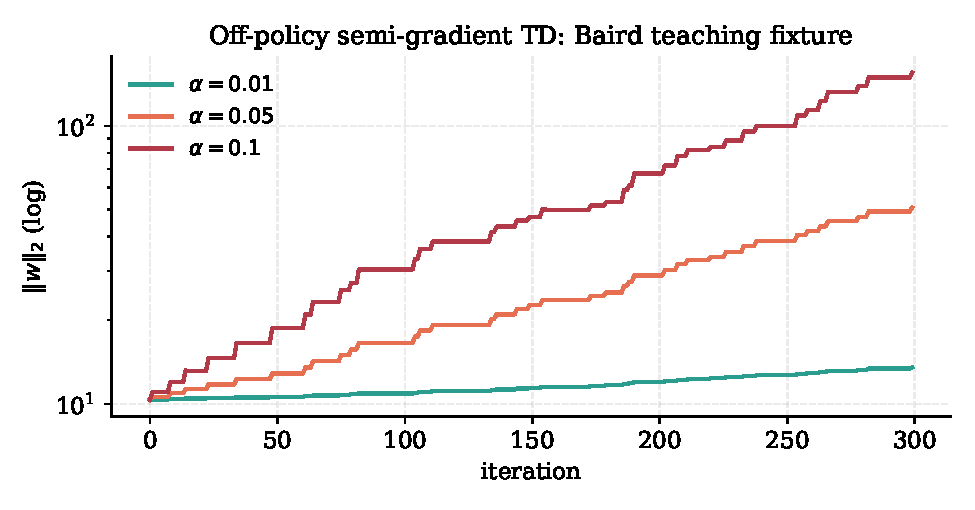
\includegraphics[width=0.85\linewidth]{figs/fig_baird_divergence.pdf}
\caption{Parameter norm under semi-gradient off-policy TD on a 7-state Baird-like
counterexample, three step sizes. All diverge; faster step size diverges faster.}
\end{figure}

\section{The DQN loss}

DQN works around the triad by (i) computing targets from a frozen copy of the network ---
the \emph{target network} $\Qfn_{\theta^-}$ updated every $C$ steps (or with Polyak
averaging $\theta^- \leftarrow (1-\tau)\theta^- + \tau\theta$); and (ii) sampling i.i.d.\
batches from a \emph{replay buffer} $\mathcal{D}$, reducing temporal
correlation between consecutive updates. Off-policy divergence can also
occur with independent samples, so decorrelation does not remove its cause.

The DQN loss for a batch $\{(s_i, a_i, r_i, s'_i, d_i)\}_{i=1}^B$ is
\begin{equation}
  \mathcal{L}(\theta) = \frac{1}{B}\sum_{i=1}^B \mathcal{L}_{\text{Huber}}\!\left(
    \Qfn_\theta(s_i, a_i),\;
    \underbrace{r_i + \Disc (1-d_i)\max_{a'} \Qfn_{\theta^-}(s'_i, a')}_{y_i}
  \right),
  \label{eq:dqn-loss}
\end{equation}
where the Huber loss
\[
  \mathcal{L}_{\text{Huber}}(x, y) = \begin{cases} \tfrac{1}{2}(x-y)^2 & |x-y| \le 1 \\ |x-y| - \tfrac{1}{2} & \text{otherwise}\end{cases}
\]
clips the gradient magnitude at large TD errors, mimicking the gradient-clip-but-keep-sign
behaviour of $\ell_1$.

\begin{theorem}[DQN gradient]
The gradient of the per-sample loss is, for the squared-error regime,
\[
  \nabla_\theta \mathcal{L}_i = -\bigl(y_i - \Qfn_\theta(s_i, a_i)\bigr)\,\nabla_\theta \Qfn_\theta(s_i, a_i).
\]
\end{theorem}

\begin{proof}
By the chain rule, treating $y_i$ as a constant (semi-gradient).
\end{proof}

\paragraph{Polyak target update.} A commonly used alternative to
hard target copies is a per-step Polyak average:
\[
  \theta^- \leftarrow (1 - \tau) \theta^- + \tau \theta, \quad \tau \approx 5\times 10^{-3}.
\]
This is what SAC, TD3, BBF and our implementation use. Hard copies (every $C=10\,000$
steps in the original DQN paper) are recovered by a time-varying $\tau$
that is zero between copies and one on copy steps, not by a fixed-$\tau$ limit.

\paragraph{Experience replay.} A circular buffer of size $|\mathcal{D}|$ (typically $10^5$
to $10^6$) stores tuples $(s, a, r, s', d)$. Each gradient step samples a uniform random
mini-batch from $\mathcal{D}$. This decorrelates updates and makes each transition usable
multiple times, raising sample efficiency. Two cost knobs: the \emph{replay ratio} (number
of gradient steps per env step, default 1 for DQN, $\ge 4$ for BBF) and the \emph{buffer
size}.

\section{Why these three tricks defang the triad}

Function approximation we cannot give up (the whole point is to generalise). Bootstrapping
we cannot give up (the whole point of TD is online learning). Off-policy sampling can break the weighting assumptions behind linear
TD stability even when consecutive samples are independent. Replay turns the data into approximate i.i.d.\
samples from $\mathcal{D}$ (still off-policy, but uncorrelated), and the target network
prevents the immediate self-reinforcement loop where a change in $\theta$ instantly
changes the target the next step pulls toward. Neither trick \emph{eliminates} divergence;
they make it much rarer for benign tasks. Adversarial tasks (Baird, multi-modal reward
landscapes, large $\Disc$ with sparse reward) still need extra care.

\begin{pitfall}
Sampling uniformly from $\mathcal{D}$ is not actually i.i.d.\ in the statistical sense:
the buffer's distribution shifts as the policy improves and old transitions evict. A
buffer that is too small produces stale targets; too large makes it slow to react to
on-policy improvements. The Sutton/Barto rule of thumb of $10^5$ on small tasks and
$10^6$ on Atari has held up.
\end{pitfall}

\section{Q-value drift and overestimation}

Two further pathologies are baked into vanilla DQN, both of which Week~6's Rainbow fixes:

\begin{enumerate}
  \item \textbf{Maximisation bias}, the same Jensen issue from Week 4. Now amplified
    because the value network is noisy in all of $\Real^8$, not just on visited table
    entries. Double-DQN (van Hasselt 2016) decouples selection and evaluation in the
    target.
  \item \textbf{Q-value drift on sparse/long-horizon tasks.} If $\Disc$ is high and the
    reward is delayed, $\Qfn$ values become large; combined with bootstrapping error,
    they keep growing. Reward clipping, distributional value heads (C51), and pop-art
    rescaling are the modern toolbox.
\end{enumerate}

\chapter{Algorithms}

\begin{algorithm}[H]
\caption{DQN (Mnih et al., 2015)}
\KwIn{learning rate $\eta$, discount $\Disc$, target update interval $C$ or Polyak $\tau$, replay capacity $|\mathcal D|$, batch size $B$}
Initialise $\theta$; copy $\theta^- \leftarrow \theta$; $\mathcal{D} \leftarrow \emptyset$\;
\For{step $= 1, 2, \ldots$}{
  Observe $s$; select $a \leftarrow \varepsilon$-greedy w.r.t.\ $\Qfn_\theta(s,\cdot)$\;
  Execute $a$, observe $(r, s', d)$\;
  Push $(s, a, r, s', d)$ into $\mathcal{D}$\;
  \If{$|\mathcal{D}| \ge$ warmup}{
    Sample batch $\{(s_i, a_i, r_i, s'_i, d_i)\}_{i=1}^B$ uniformly from $\mathcal{D}$\;
    Compute targets $y_i = r_i + \Disc (1 - d_i) \max_{a'} \Qfn_{\theta^-}(s'_i, a')$\;
    Compute loss $\mathcal{L} = \frac{1}{B}\sum_i \mathcal{L}_{\text{Huber}}(\Qfn_\theta(s_i, a_i), y_i)$\;
    Step: $\theta \leftarrow \theta - \eta \nabla_\theta \mathcal{L}$ (with grad-norm clip 10)\;
    \If{Polyak}{$\theta^- \leftarrow (1-\tau)\theta^- + \tau\theta$}
    \ElseIf{step $\equiv 0 \pmod C$}{$\theta^- \leftarrow \theta$}
  }
}
\end{algorithm}

\paragraph{Complexity.} Per env step: one forward pass on the policy net (for $a$), one
batch forward-backward on the policy net + one forward on the target net for learning.
Memory: $|\mathcal D| \cdot (2 \cdot \dim(\States) + 3)$ floats for the buffer, plus
network params. On LunarLander (8-D obs) a $10^5$ buffer is roughly 6.5 MB; on Atari (84
x 84 x 4 uint8 frames) the same is roughly 7 GB and requires stacking and frame skipping.

\begin{example}[A worked DQN step on LunarLander]
$s = (1.2, 0.5, 0.0, 0.0, -0.1, 0.0, 0, 0)$ (centred, mid-air). $a = 2$ (main engine).
$(r, s', d) = (-0.1, (\ldots), \text{False})$. Forward-pass: $\Qfn_\theta(s) = [0.4, 1.1,
2.0, 0.7]$ so $\Qfn_\theta(s, 2) = 2.0$. Target net: $\Qfn_{\theta^-}(s') = [0.5, 1.2, 2.1,
0.8]$ so $\max = 2.1$, $y = -0.1 + 0.99 \cdot 2.1 = 1.979$. TD error $\delta = 1.979 - 2.0
= -0.021$. Huber on $|\delta| < 1$ collapses to $\tfrac{1}{2}\delta^2 \approx 2 \times
10^{-4}$. Gradient step pushes $\Qfn_\theta(s, 2)$ slightly down.
\end{example}

\begin{pitfall}
The single most common DQN bug is using \texttt{terminated} interchangeably with
\texttt{truncated}. For an artificial time-limit truncation in a continuing task, retain the
bootstrap from the final observation. For a true terminal transition, remove
it. Keep both booleans: use either to end collection, but only true
termination to zero the continuation value. A reset observation must not
replace the final observation in the bootstrap.
\end{pitfall}

\chapter{Implementation walkthrough}

The reference agent is in \texttt{project/agent.py}. Core fragments:

\begin{minted}{python}
class DQNAgent:
    def learn(self) -> float | None:
        if len(self.buf) < max(self.cfg.batch_size, self.cfg.warmup_steps):
            self.step_count += 1
            return None
        s, a, r, s2, d = self.buf.sample(self.cfg.batch_size)
        s  = torch.as_tensor(s, device=self.cfg.device)
        a  = torch.as_tensor(a, dtype=torch.long, device=self.cfg.device)
        r  = torch.as_tensor(r, device=self.cfg.device)
        s2 = torch.as_tensor(s2, device=self.cfg.device)
        d  = torch.as_tensor(d, device=self.cfg.device)
        q_sa = self.q(s).gather(1, a.unsqueeze(1)).squeeze(1)
        with torch.no_grad():
            q_next = self.q_target(s2).max(dim=1).values
            target = r + (1.0 - d) * self.cfg.gamma * q_next
        loss = F.smooth_l1_loss(q_sa, target)
        self.opt.zero_grad(); loss.backward()
        torch.nn.utils.clip_grad_norm_(self.q.parameters(), self.cfg.grad_clip)
        self.opt.step()
        self._soft_update()
        self.step_count += 1
        return float(loss.item())
\end{minted}

The exploration schedule is a linear decay (Mnih 2015 used $\varepsilon: 1.0 \to 0.1$ over
1M frames; we use a shorter $30$k steps for LunarLander):

\begin{minted}{python}
def epsilon(self) -> float:
    if self.step_count >= self.cfg.eps_decay_steps:
        return self.cfg.eps_end
    frac = self.step_count / self.cfg.eps_decay_steps
    return self.cfg.eps_start + (self.cfg.eps_end - self.cfg.eps_start) * frac
\end{minted}

The replay buffer reuses \texttt{common/replay.py} from earlier weeks.

\begin{pitfall}
Two implementation traps cost most beginners a day each:
\textbf{(i)} forgetting to put $\theta^-$ in \texttt{torch.no\_grad()} and watching memory
balloon as autograd builds a graph through the target;
\textbf{(ii)} using \texttt{.gather(1, a)} without first \texttt{.unsqueeze(1)} on the
action tensor, silently picking $\Qfn(s,a_0)$ for all batch elements.
\end{pitfall}

\chapter{Empirical results}

\begin{figure}[h]
\centering
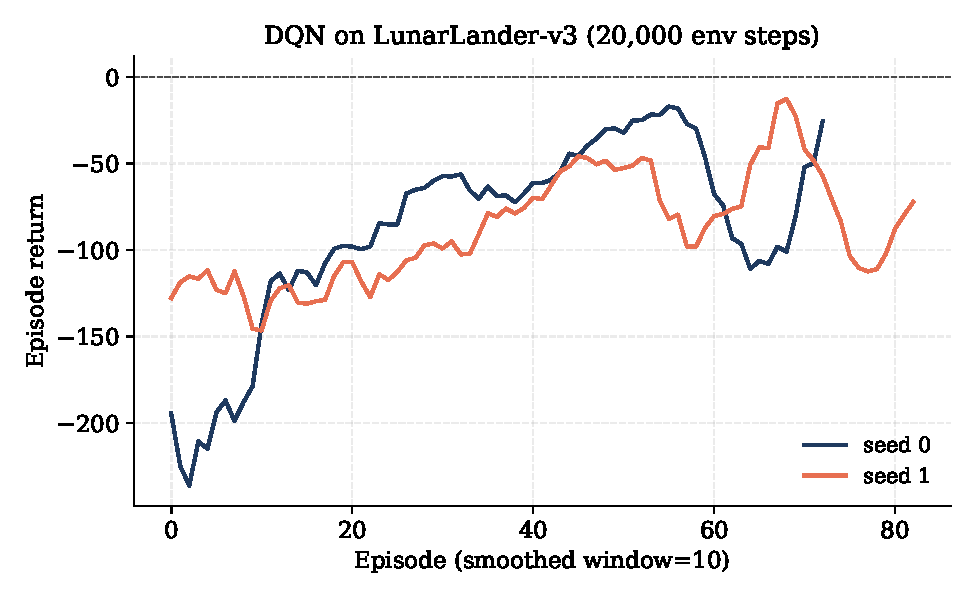
\includegraphics[width=0.95\linewidth]{figs/fig_dqn_lunar_curve.pdf}
\caption{Historical DQN run on LunarLander-v3 (20k environment steps, 2 seeds).
This finite experiment illustrates episode-return variation; it does not
certify convergence or guarantee the full-training target. The current
trainer retains bootstrapping at external time-limit truncations.}
\end{figure}

\begin{figure}[h]
\centering
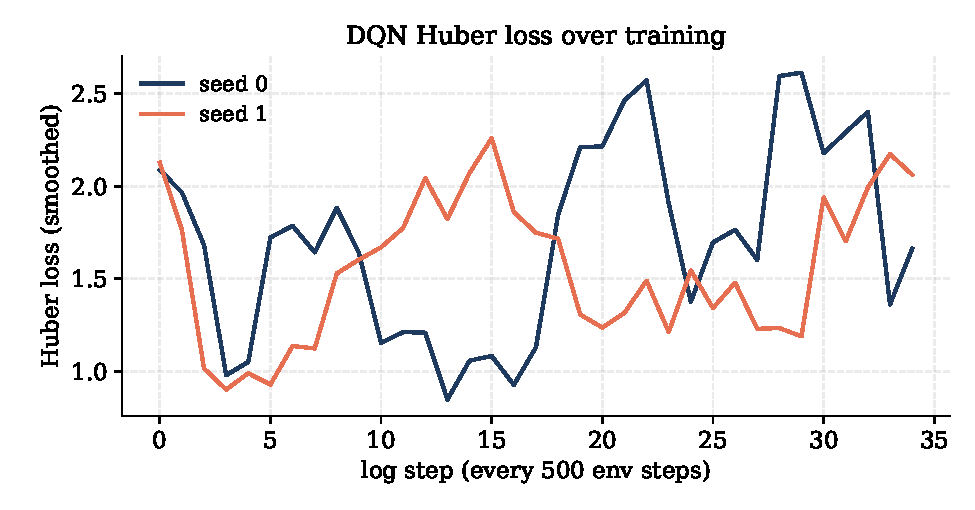
\includegraphics[width=0.95\linewidth]{figs/fig_dqn_loss.pdf}
\caption{Huber loss over training. Note the spikes: each one corresponds to the agent
discovering a new high-reward region of state-action space where the existing $\Qfn$ is
maximally wrong. Such spikes are normal --- the long-run trend matters.}
\end{figure}

\begin{figure}[h]
\centering
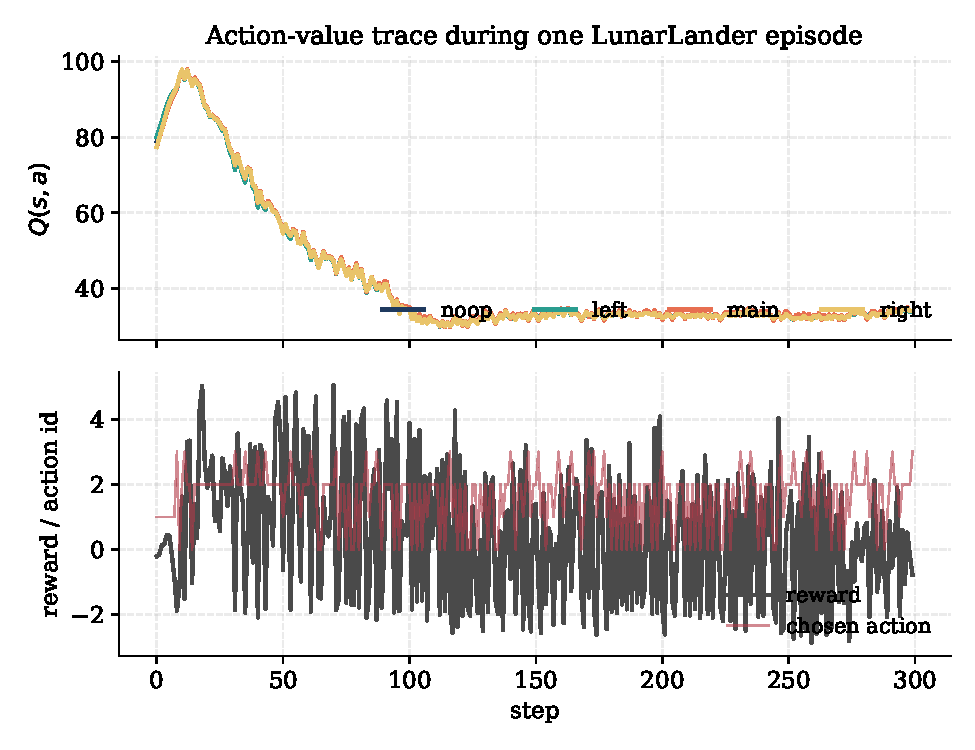
\includegraphics[width=0.95\linewidth]{figs/fig_dqn_qtrace.pdf}
\caption{Top: $\Qfn(s, a)$ for each of the four actions during one greedy rollout. The
four curves are tightly coupled when the lander is far from the pad (state is easy ---
small differences) and diverge near landing where action choice matters. Bottom: the
chosen action overlaid with the realised reward.}
\end{figure}

\begin{safetyangle}
\textbf{The deadly triad as a safety pathology.}
The triad is not just an academic curiosity; its three concrete clinical manifestations
are exactly the failure modes that bite in a deployed safety-critical agent:

\begin{enumerate}
  \item \textbf{Q-value drift in deployment.} A safety-critical agent left learning
    online with a too-large replay buffer can encounter a slow drift in $\Qfn$ values
    that silently degrades policy quality before any reward signal can catch it. The
    canonical fix is a \emph{frozen safe baseline} that is only updated after offline
    re-evaluation passes a bar --- the pattern Weeks 14--15 (offline RL) and Week~24
    (capstone) develop in full.
  \item \textbf{Divergence on distribution shift.} Off-policy + function approximation is
    exactly the regime where a new operating mode (a new lead segment, a new robot
    payload) silently violates the i.i.d.\ replay assumption. Conservative Q-learning
    (CQL, Kumar 2020) and IQL (Kostrikov 2022) penalise out-of-distribution actions
    explicitly to bound this.
  \item \textbf{Optimism near catastrophes.} The max-bias of vanilla Q-learning is a
    one-way error: it overestimates. In a high-cost-asymmetric environment (cliff, robot
    arm, dose-response) this means the agent's miscalibration always pushes it toward
    the catastrophe. Distributional value heads (C51, IQN; Week 6) let you read out the
    lower CVaR of the return distribution and pick risk-averse policies; CMDPs (Week 22)
    install hard budgets.
\end{enumerate}
Reference: see \texttt{research/safety\_rl\_sota.md} \S3 (Risk-Sensitive RL: CVaR and
Distributional Approaches) for the full risk-sensitive story.
\end{safetyangle}

\begin{matching}
\textbf{From CliffWalking-Q to LunarLander-DQN to lead matching.}
The week's mini-project is a single agent in a single environment, but the abstraction it
teaches transfers directly: any insurance/recruitment lead-routing system with a numerical
feature vector per lead can be cast as $\States = \Real^d$, $\Actions = \{\text{broker}_1,
\ldots, \text{broker}_K\}$, $r$ = signed margin of conversion. Pre-trained DQN gives a
stationary policy that ranks brokers per lead. Two practical deltas from LunarLander to
the matching setting:
\begin{itemize}
  \item The MDP is degenerate (each lead is one step); we are doing contextual
    \emph{bandits} not full RL. Set $\Disc = 0$ and the DQN target collapses to standard
    regression on $r$. We will spend Week~11 on the proper formalism (LinUCB, Thompson
    Sampling, doubly-robust OPE) but DQN-with-$\Disc=0$ is a perfectly serviceable
    baseline.
  \item Action-availability \emph{varies} per lead (broker capacity, geographic match).
    Use \emph{action masking}: set $\Qfn(s, a_\text{invalid}) = -\infty$ before the
    argmax. Masking prevents selection of that action, but does not remove the deadly triad or ensure stable value learning
    under both behaviour and target.
\end{itemize}
\end{matching}

\chapter{Exercises}

The graded workbook (\texttt{workbook.ipynb}) has 9 exercises:

\begin{enumerate}
  \item Gather $\Qfn(s,a)$ from a batched network output ($\bigstar$).
  \item DQN bootstrap target with the done-mask ($\bigstar\bigstar$).
  \item Polyak soft target update ($\bigstar$).
  \item $\varepsilon$-greedy action selection from a Q-net ($\bigstar$).
  \item Per-element TD error for PER prioritisation ($\bigstar\bigstar$).
  \item Huber/smooth-L1 loss ($\bigstar$).
  \item Reproduce Baird's divergence ($\bigstar\bigstar\bigstar$).
  \item Smoke training pass on LunarLander ($\bigstar\bigstar$).
  \item Action-value trace visualisation across an episode ($\bigstar\bigstar\bigstar$, meaningful objective).
\end{enumerate}

\chapter{Further reading}

\texttt{extended\_reading.pdf} covers Mnih et al.\ 2015 (DQN \emph{Nature}), Mnih et al.\
2013 (DQN NeurIPS workshop), Sutton \& Barto 11.3 (the deadly triad), Baird 1995, and
Farebrother et al.\ 2018 (generalisation gap in DQN). For the engineering best-practice
trail of 2024--2026 see \texttt{research/deeprl\_core\_sota.md} \S1 (DQN family).

\end{document}
